\documentclass[14pt]{beamer}

\usetheme{simple}

\usepackage[utf8]{inputenc}
\usepackage[light,sfdefault]{roboto}
\usepackage{color}
% https://tex.stackexchange.com/questions/23711/strikethrough-text
\usepackage{soul}
\usepackage{tikz}
\usepackage{makecell}
\usepackage{xcolor}
\usepackage[%
  font=normalsize,
  labelfont=normalsize,
  justification=centering
]{caption}

\definecolor{MPIgreen}{RGB}{66,135,59}

\usetikzlibrary{arrows.new}
\tikzset{arrow/.style={-latex new,arrow head=0.25cm}}

\title{PointNet: Deep Learning on Point Sets for 3D Classification and Segmentation \cite{GarciaGarcia:2016}}
\author{David Stutz}
\date{June 1-2, 2017}

\begin{document}
  \begin{frame}[plain]
    \titlepage
  \end{frame}

  \begin{frame}
    \frametitle{Motivation}
    Which is the best 3D representation for deep learning?
    \begin{itemize}
      \item Voxel grids,
      \item triangular meshes,
      \item point clouds,
      \item projections ...
    \end{itemize}
    \vskip 1em
    
    How to efficiently train deep models on 3D data?
    \begin{itemize}
      \item Efficient convolutions (e.g. \cite{Engelcke:2016}),
      \item efficient data structures (e.g. OctNets \cite{Riegler:2016,Riegler:2017,Tatarchenko:2017,Wang:2017}) ...
    \end{itemize}
  \end{frame}
  
  \begin{frame}
    \frametitle{Related Work}
    {\footnotesize
    \fbox{
    \begin{minipage}[t][3cm][t]{0.45\textwidth}
      ``Traditional'' 3D CNNs\\
      (\cite{Maturana:2015,Sharma:2016,Chen:2016,Hegde:2016,Sedaghat:2016,Li:2016,Qi:2016,Wu:2014,Girdhar:2016} ...)
      \begin{itemize}
        \item Meshes or point clouds are voxelized;
        \item efficient convolution possible \cite{Engelcke:2016}.
      \end{itemize}
    \end{minipage}
    }
    \hfill
    \phantom{
    \fbox{
    \begin{minipage}[t][3cm][t]{0.45\textwidth}
      Efficient Data Structure\\
      (\cite{Riegler:2016,Riegler:2017,Tatarchenko:2017,Wang:2017})
      \begin{itemize}
        \item Octree-based,
        \item learning structure difficult.
      \end{itemize}
    \end{minipage}
    }
    }
    \vskip 0.2cm
    \phantom{
    \fbox{
    \begin{minipage}[t][3cm][t]{0.45\textwidth}
      ``Manifold'' CNNs\\
      (\cite{Masci:2015} -- more?)
      \begin{itemize}
        \item Extends Euclidean CNNs to Riemannian manifolds.
      \end{itemize}
    \end{minipage}
    }
    }
    \hfill
    \phantom{
    \fbox{
    \begin{minipage}[t][3cm][t]{0.45\textwidth}
      Point Clouds\\
      (\cite{Fan:2016,GarciaGarcia:2016})
      \begin{itemize}
        \item Sample points from meshes;
        \item operate directly on unordered point sets.
      \end{itemize}
    \end{minipage}
    }
    }
    }
  \end{frame}
  
  \begin{frame}
    \frametitle{Related Work}
    {\footnotesize
    \fbox{
    \begin{minipage}[t][3cm][t]{0.45\textwidth}
      ``Traditional'' 3D CNNs\\
      (\cite{Maturana:2015,Sharma:2016,Chen:2016,Hegde:2016,Sedaghat:2016,Li:2016,Qi:2016,Wu:2014,Girdhar:2016} ...)
      \begin{itemize}
        \item Meshes or point clouds are voxelized;
        \item efficient convolution possible \cite{Engelcke:2016}.
      \end{itemize}
    \end{minipage}
    }
    \hfill
    \fbox{
    \begin{minipage}[t][3cm][t]{0.45\textwidth}
      Efficient Data Structure\\
      (\cite{Riegler:2016,Riegler:2017,Tatarchenko:2017,Wang:2017})
      \begin{itemize}
        \item Octree-based,
        \item learning structure difficult.
      \end{itemize}
    \end{minipage}
    }
    \vskip 0.2cm
    \phantom{
    \fbox{
    \begin{minipage}[t][3cm][t]{0.45\textwidth}
      ``Manifold'' CNNs\\
      (\cite{Masci:2015} -- more?)
      \begin{itemize}
        \item Extends Euclidean CNNs to Riemannian manifolds.
      \end{itemize}
    \end{minipage}
    }
    }
    \hfill
    \phantom{
    \fbox{
    \begin{minipage}[t][3cm][t]{0.45\textwidth}
      Point Clouds\\
      (\cite{Fan:2016,GarciaGarcia:2016})
      \begin{itemize}
        \item Sample points from meshes;
        \item operate directly on unordered point sets.
      \end{itemize}
    \end{minipage}
    }
    }
    }
  \end{frame}
  
  \begin{frame}
    \frametitle{Related Work}
    {\footnotesize
    \fbox{
    \begin{minipage}[t][3cm][t]{0.45\textwidth}
      ``Traditional'' 3D CNNs\\
      (\cite{Maturana:2015,Sharma:2016,Chen:2016,Hegde:2016,Sedaghat:2016,Li:2016,Qi:2016,Wu:2014,Girdhar:2016} ...)
      \begin{itemize}
        \item Meshes or point clouds are voxelized;
        \item efficient convolution possible \cite{Engelcke:2016}.
      \end{itemize}
    \end{minipage}
    }
    \hfill
    \fbox{
    \begin{minipage}[t][3cm][t]{0.45\textwidth}
      Efficient Data Structure\\
      (\cite{Riegler:2016,Riegler:2017,Tatarchenko:2017,Wang:2017})
      \begin{itemize}
        \item Octree-based,
        \item learning structure difficult.
      \end{itemize}
    \end{minipage}
    }
    \vskip 0.2cm
    \fbox{
    \begin{minipage}[t][3cm][t]{0.45\textwidth}
      ``Manifold'' CNNs\\
      (\cite{Masci:2015} -- more?)
      \begin{itemize}
        \item Extends Euclidean CNNs to Riemannian manifolds.
      \end{itemize}
    \end{minipage}
    }
    \hfill
    \phantom{
    \fbox{
    \begin{minipage}[t][3cm][t]{0.45\textwidth}
      Point Clouds\\
      (\cite{Fan:2016,GarciaGarcia:2016})
      \begin{itemize}
        \item Sample points from meshes;
        \item operate directly on unordered point sets.
      \end{itemize}
    \end{minipage}
    }
    }
    }
  \end{frame}
  
  \begin{frame}
    \frametitle{Related Work}
    {\footnotesize
    \fbox{
    \begin{minipage}[t][3cm][t]{0.45\textwidth}
      ``Traditional'' 3D CNNs\\
      (\cite{Maturana:2015,Sharma:2016,Chen:2016,Hegde:2016,Sedaghat:2016,Li:2016,Qi:2016,Wu:2014,Girdhar:2016} ...)
      \begin{itemize}
        \item Meshes or point clouds are voxelized;
        \item efficient convolution possible \cite{Engelcke:2016}.
      \end{itemize}
    \end{minipage}
    }
    \hfill
    \fbox{
    \begin{minipage}[t][3cm][t]{0.45\textwidth}
      Efficient Data Structure\\
      (\cite{Riegler:2016,Riegler:2017,Tatarchenko:2017,Wang:2017})
      \begin{itemize}
        \item Octree-based,
        \item learning structure difficult.
      \end{itemize}
    \end{minipage}
    }
    \vskip 0.2cm
    \fbox{
    \begin{minipage}[t][3cm][t]{0.45\textwidth}
      ``Manifold'' CNNs\\
      (\cite{Masci:2015} -- more?)
      \begin{itemize}
        \item Extends Euclidean CNNs to Riemannian manifolds.
      \end{itemize}
    \end{minipage}
    }
    \hfill
    \fbox{
    \begin{minipage}[t][3cm][t]{0.45\textwidth}
      Point Clouds\\
      (\cite{Fan:2016,GarciaGarcia:2016})
      \begin{itemize}
        \item Sample points from meshes;
        \item operate directly on unordered point sets.
      \end{itemize}
    \end{minipage}
    }
    }
  \end{frame}
  
  \begin{frame}
    \frametitle{Point Set Properties}
    Consider point set $\{x_1, \ldots, x_n\} \subseteq \mathbb{R}^3$:
    \begin{itemize}
      \item unordered: in contrast to voxel grids no inherent order -- invariance to $n!$ permutations required;
      \item distance metric: interactions between points through a distance on $\mathbb{R}^3$;
      \item invariance: invariance to 3D transformations required.
    \end{itemize}
  \end{frame}
  
  \begin{frame}
    \frametitle{Unordered Point Sets}
    Goal: invariance to $n!$ permutations.
    \vskip 1em
    Idea:
    \begin{align}
      f(\{x_1,\ldots,x_n\}) \approx g(h(x_1),\ldots,h(x_n))\notag
    \end{align}
    \tikz[overlay]{
      \draw[MPIgreen,arrow] (9,0.25) node{feature transform} (7,0.25) [out=180,in=290]to (5.95,0.9);
      \draw[MPIgreen,arrow] (2,0.25) node{symmetric function} (4.25,0.25) [out=0,in=270]to (5.35,0.9);
    }
    \vskip 1em
    In practice:
    \begin{itemize}
      \item $h(x)$ modeled as multi-layer perceptron;
      \item $g = \max$.
    \end{itemize}
  \end{frame}
  
  \begin{frame}
    \frametitle{Unordered Point Sets (cont'd)}
    Theorem (informal): any continuous function can be approximated as
    \begin{align}
      f(\{x_1,\ldots,x_n\}) \approx \max(h(x_1),\ldots,h(x_n)).\notag
    \end{align}
    \vskip 1em
    
    Further result: ``Intuitively, our network learns to summarize shape by a sparse set of key points''.
    \begin{itemize}
      \item It exists a critical set of points.
    \end{itemize}
  \end{frame}
  
  \begin{frame}
    \frametitle{Invariances}
    Goal: learn invariances regarding rotations, translations, noise ...
    \vskip 1em
    Idea: joint alignment network ...
    \begin{figure}
      \centering
      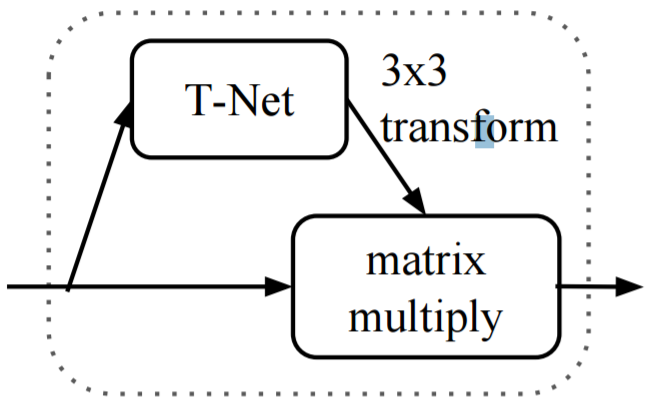
\includegraphics[scale=0.5]{alignment_network}
    \end{figure}
  \end{frame}
  
  \begin{frame}
    \frametitle{Shape Classification}
    \begin{figure}
      \centering
      \hspace*{-0.5cm}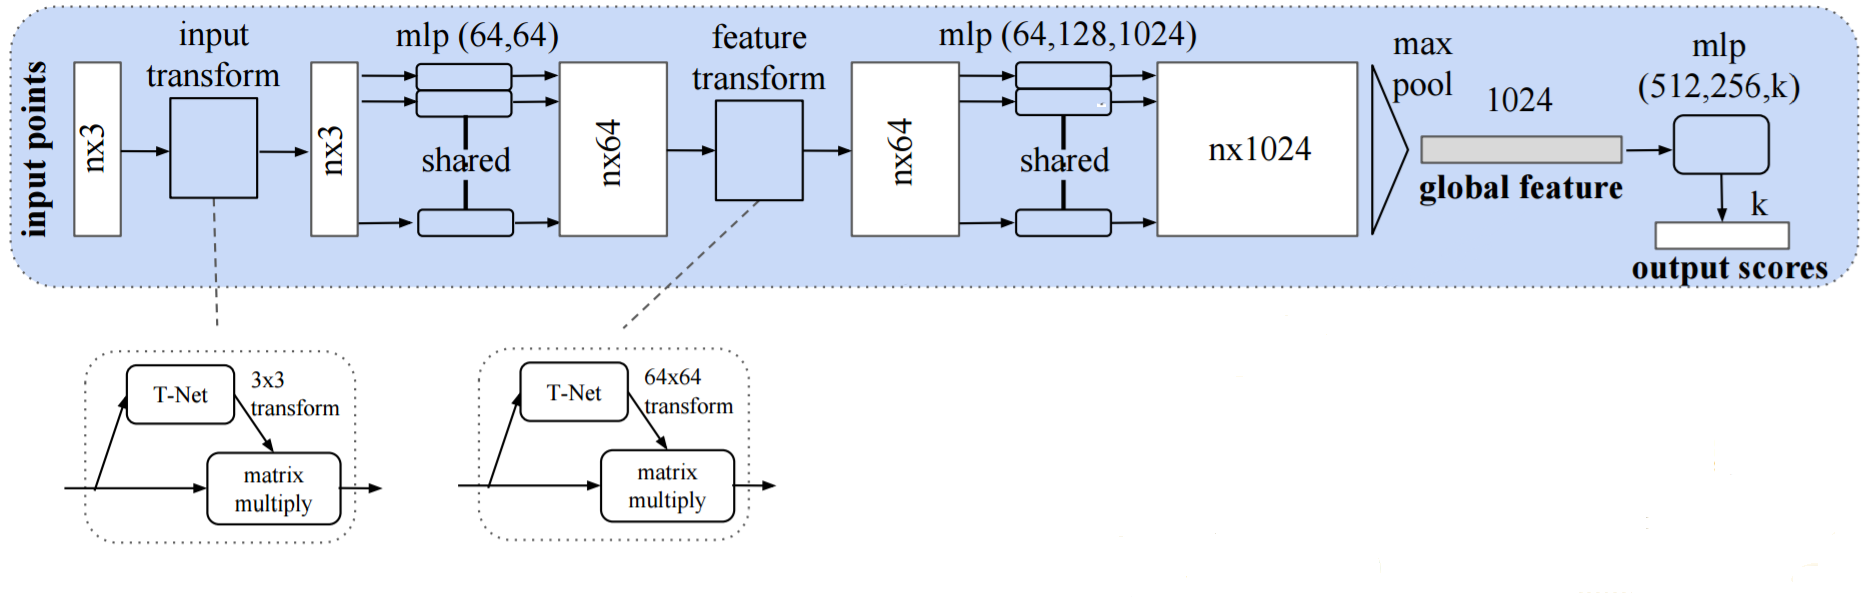
\includegraphics[scale=0.3]{classification_network}
    \end{figure}  
  \end{frame}
  
  \begin{frame}
    \frametitle{Shape Classification (cont'd)}
    Experimental setup:
    \begin{itemize}
      \item ModelNet40 \cite{Wu:2014};
      \item $1024$ sampled points;
      \item normalized to unit sphere;
      \item randomly rotated;
      \item with Gaussian noise ($\sigma = 0.02$).
    \end{itemize}
  \end{frame}
  
  \begin{frame}
    \frametitle{Shape Classification (cont'd)}
    \begin{table}
      {\renewcommand*{\arraystretch}{1}
      \begin{tabular}{l | c | c c}
        &  & \makecell{overall\\accuracy} & \makecell{average\\class\\accuracy}\\\hline
        VoxNet \cite{Maturana:2015} & volumes & 83 & 85.9\\
        Subvolume \cite{Qi:2016} & volumes & 86 & 89.2\\
        MVCNN \cite{Su:2015} & images & -- & 90.1\\
        PointNet & points & 89.2 & 86.2\\
      \end{tabular}
      }
      \tikz[overlay]{
        \draw[MPIgreen,arrow] (1,-1.5) node{numbers hard to trace in literature} (5,-1.5) [out=0,in=335] to (5,1);
      }
      \caption{Accuracy on ModelNet40.}
    \end{table}
  \end{frame}
  
  \begin{frame}
    \frametitle{Shape Classification (cont'd)}
    \vskip 1em
    \begin{figure}
      \centering
      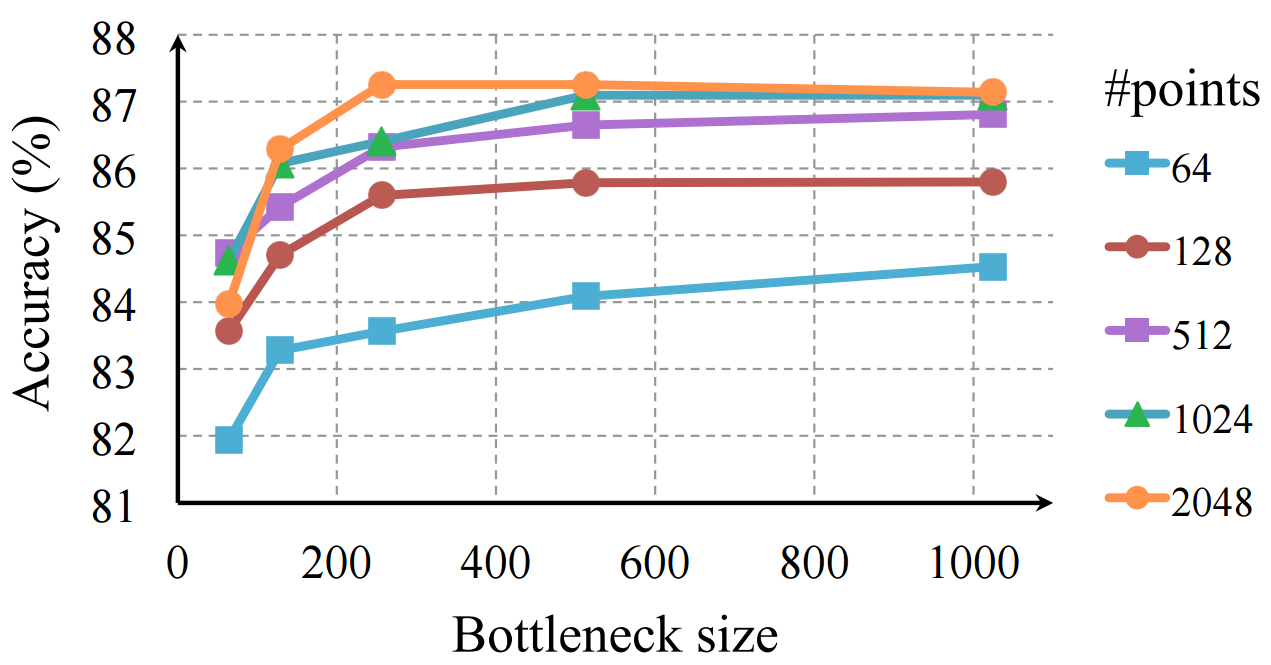
\includegraphics[scale=0.3]{bottleneck_size}
      \caption{Overall accuracy on ModelNet40.}
      \tikz[overlay]{
        \draw[MPIgreen,arrow] (0,7) node{green one should be 89.2} (3,7) [out=0,in=15] to (3,6.05);
      }
    \end{figure}  
  \end{frame}
  
  \begin{frame}
    \frametitle{Critical Sets}
    \begin{figure}
      \centering
      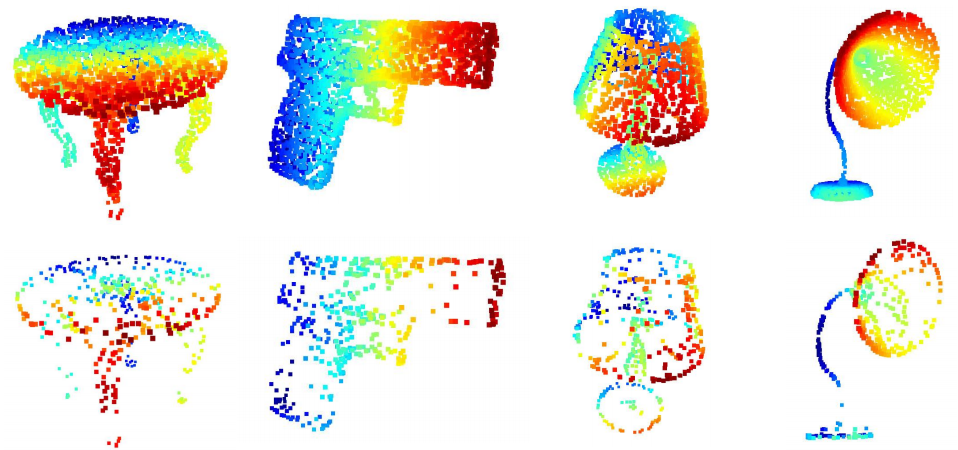
\includegraphics[scale=0.425]{critical_sets}
      \caption{Critical point sets, i.e. points that contribute to the max-pooling features.}
    \end{figure}
  \end{frame}
  
  \begin{frame}
    \frametitle{My 2 Cents ...}
    Revisiting properties of point sets:
    \begin{itemize}
      \item \only<1>{unordered}\only<2->{\st{unordered} symmetric function \checkmark};
      \item \only<1->{interactions between points}\only<3->{?};
      \item \only<1-3>{invariances}\only<4->{\st{invariances} alignment network \checkmark};
    \end{itemize}
  \end{frame}
  
  \begin{frame}
    \frametitle{My 2 Cents ... (cont'd)}
    For meshes:
    \begin{itemize}
      \item additional local structure (faces) available;
      \item invariance to points sampled from the same mesh;
      \item no notion of ``surface'' without point normals.
    \end{itemize}
  \end{frame}
  
  \begin{frame}
    \frametitle{Conclusion}
    PointNet = (shared) multilayer perceptrons on individual points + max pooling over points.
    \vskip 1em
    
    Interesting alternative to OctNets to apply deep learning on sparse 3D data.
    \begin{itemize}
      \item Still some open questions to investigate ...
    \end{itemize}
  \end{frame}
  
  \begin{frame}[allowframebreaks]
    \frametitle{References}
    \bibliography{slides} 
    \bibliographystyle{plain}
  \end{frame}
\end{document}
